%%%%%%%%%%%%%%%%%%%%%%%%%%%%%%%%%%%%%%%%%%%%%%
% Analysis
%%%%%%%%%%%%%%%%%%%%%%%%%%%%%%%%%%%%%%%%%%%%%%
\section{Analysis}\label{sec:analysis}

\subsection{Network Analysis}\label{sec:network_analysis}
% Get numbers from Dashboard + Images
\begin{figure}[H]
  \begin{center}
    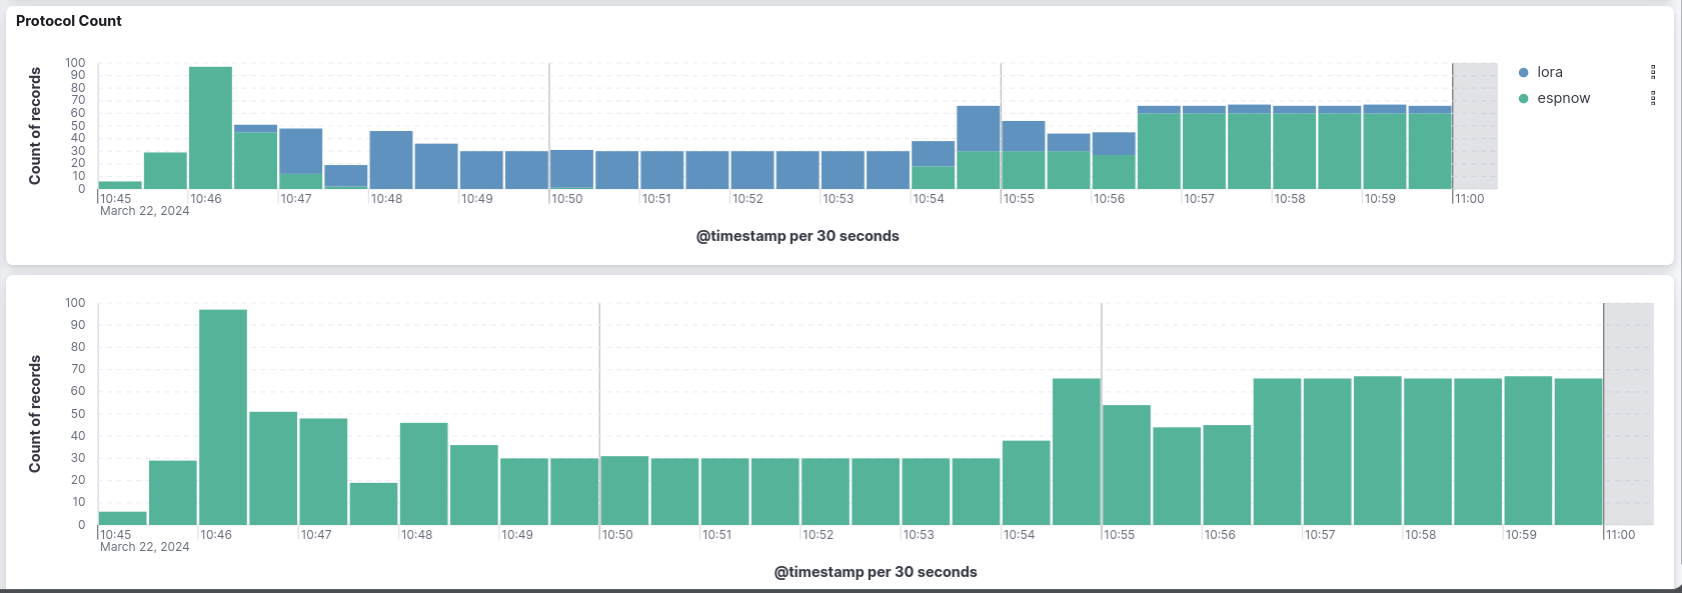
\includegraphics[width=0.45\textwidth]{./Figures/elk/protocol_count.png}
  \end{center}
  \caption{Protocol Distribution}\label{fig:protocol_distribution}
\end{figure}

Figure \ref{fig:protocol_distribution} delineates the distribution of transmitted packets across the LoRa and ESP-Now protocols. The graph portrays LoRa Packets denoted in blue and ESP-Now Packets in green in the Protocol Count-Time Graph (Top). Evidently, the ESP-Now protocol emerges as the predominant choice, exhibiting a higher packet count vis-à-vis the LoRa protocol in the Count of records-Time Graph (bottom).

The discernible instances of protocol switching, notably observed around the timestamps 10:46 and 10:54, underscore the dynamic nature of the implemented ESP-Now Mesh and LoRa Mesh. During these transitions, a shift from LoRa to ESP-Now and vice versa is perceptible, as delineated by the transitions between the blue and green segments in the graph.

All calculations are based on the figures depicted in Figure \ref{fig:espnowthroughput} for ESP-NOW throughput and Figure \ref{fig:lorathroughput} for LoRa throughput. These figures represent the packets received by the Master node in a network configuration consisting of 4 nodes arranged in a linear topology with 4 levels of hopping. The timing intervals for data collection were approximately 60 minutes for ESP-NOW and 50 minutes for LoRa Mesh.

\begin{figure}[H]
  \begin{center}
    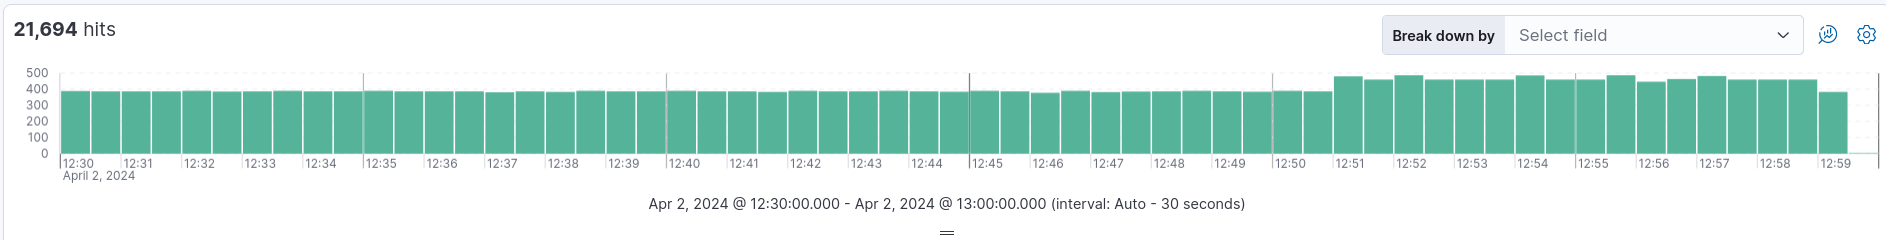
\includegraphics[width=0.45\textwidth]{./Figures/elk/espnow.png}
  \end{center}
  \caption{ESP NOW Throughput}\label{fig:espnowthroughput}
\end{figure}

\begin{figure}[H]
  \begin{center}
    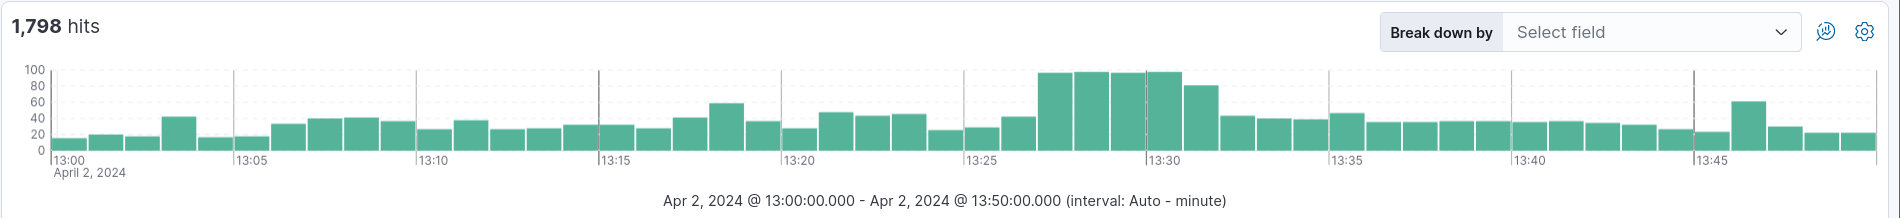
\includegraphics[width=0.45\textwidth]{./Figures/elk/lora.png}
  \end{center}
  \caption{LoRa Throughput}\label{fig:lorathroughput}
\end{figure}

Figure \ref{fig:espnowthroughput} illustrates the received ESP-NOW packets, while Figure \ref{fig:lorathroughput} displays the received LoRa packets. These visualizations provide insights into the performance of each protocol within the network configuration.

The data collected from these figures serves as the basis for calculating various network metrics, including throughput, latency, and bandwidth, which are essential for evaluating the efficiency and effectiveness of the communication protocols in the network.

Note that the extra multiple of 3 is used to scale the LoRa data to fit the same time delay implemented in the ESP-NOW Mesh (1 Second for ESP-NOW vs 3 second for LoRa).

\subsubsection{Throughput Calculation:}

To calculate the throughput of our mesh network, we utilized the formula:

\[
\text{throughput} = \frac{\text{total packets received}}{\text{Total time (seconds)}}
\]

For ESP NOW:

\[
\text{throughput} = \frac{21694}{60 \cdot 60} \approx 6.0261 \text{ packets/second}
\]

For LoRa:

\[
\text{throughput} = \frac{1789}{60 \cdot 50} \cdot 3 \approx 1.789 \text{ packets/second}
\]

ESP NOW achieves a throughput of approximately 6.0261 packets per second, indicating its capability to handle a higher volume of data compared to LoRa. Despite LoRa's lower throughput of approximately 1.789 packets per second, it is known for its extended range and superior penetration through obstacles. Therefore, while ESP NOW excels in terms of raw data transmission rate, LoRa's strengths lie in its ability to maintain connectivity over longer distances and in challenging environments.

\subsubsection{Latency Calculation:}

To calculate latency, we use the formula:

\[
\text{Latency} = \frac{\text{Total time (seconds)}}{\text{total packets received}}
\]

For ESP NOW:
\[
\text{Latency} = \frac{60 \cdot 60}{21694} \approx 0.165 \text{ seconds/packet}
\]

For LoRa:
\[
\text{Latency} = \frac{60 \cdot 50}{1789} \cdot 3 \approx 1.676 \text{ seconds/packet}
\]

Latency represents the time it takes for a packet to travel from the sender to the receiver in the network.

For ESP NOW, the latency is approximately 0.165 seconds per packet.

For LoRa, the latency is approximately 1.676 seconds per packet.

Comparing both results, ESP NOW exhibits significantly lower latency compared to LoRa, making it more suitable for applications requiring real-time or low-latency communication.

\subsubsection{Bandwidth Calculation:}

Bandwidth is calculated using the formula:

\[
\text{Bandwidth} = \frac{\text{Packet Count} \cdot \text{Packet Size}}{\text{Total time (seconds)}}
\]

For ESP NOW:
\[
\text{Bandwidth} = \frac{21694 \cdot 30 \text{ bytes}}{60 \cdot 60} \approx 180.78 \text{ (in bytes/second)}
\]

For LoRa:
\[
\text{Bandwidth} = \frac{1789 \cdot 50 \text{ bytes}}{60 \cdot 50} \cdot 3 \approx 89.45 \text{ (in bytes/second)}
\]

Bandwidth quantifies the rate at which data is transmitted over the network.

For ESP NOW, the calculated bandwidth is approximately 180.78 bits per second.

For LoRa, the calculated bandwidth is approximately 89.45 bits per second.

Comparing both results, ESP NOW demonstrates higher bandwidth compared to LoRa. This indicates that ESP NOW is capable of transmitting data at a faster rate, making it advantageous for applications requiring high data throughput.

\subsubsection{Network analysis summary}

The comparison between LoRa and ESP NOW in the context of a Wireless Sensor Network (WSN) with 4 nodes in a line and 1 master reveals distinct performance characteristics. ESP NOW demonstrates significantly higher throughput, achieving approximately 6.0261 packets per second, compared to LoRa's throughput of approximately 1.789 packets per second. However, this higher throughput comes at the expense of increased latency, with ESP NOW exhibiting a latency of approximately 0.165 seconds per packet, while LoRa has a latency of approximately 1.676 seconds per packet. Furthermore, when considering bandwidth, ESP NOW provides higher bandwidth at approximately 180.78 bytes per second, whereas LoRa's bandwidth is approximately 89.45 bytes per second. Therefore, while ESP NOW offers superior throughput and bandwidth, LoRa presents advantages in terms of latency and potentially longer range and better obstacle penetration, making it a more suitable choice for scenarios prioritizing these factors.




% ESP NOW: 21694/ (60*60) = 6.0261 packets/second
% LORA: (1789/ 60*50) + 3 = 1.789 packets per scond


% An intriguing observation pertains to the periodic dips in bandwidth, indicative of intervals where the network experiences a diminished packet reception rate. Plausible factors contributing to this phenomenon encompass variances in protocol efficiency or disparities in mesh implementation. Despite both protocols being instantiated with the DSR mesh algorithm, the Lora protocol potentially suffers from a lower packet reception rate owing to its inherent characteristics, including a lower data rate and extended transmission range.


% Total packet count / total time (seconds)

% Jovian section
\subsection{ESP-NOW vs LORA Power Consumption Analysis}\label{sec:power_consumption_analysis}
The following segment presents an analysis of the power utilization contrasts between ESP-NOW and LoRa nodes, alongside a comparative study of the master nodes for both ESP-NOW and LoRa protocols.

\begin{figure}[H]
  \begin{center}
    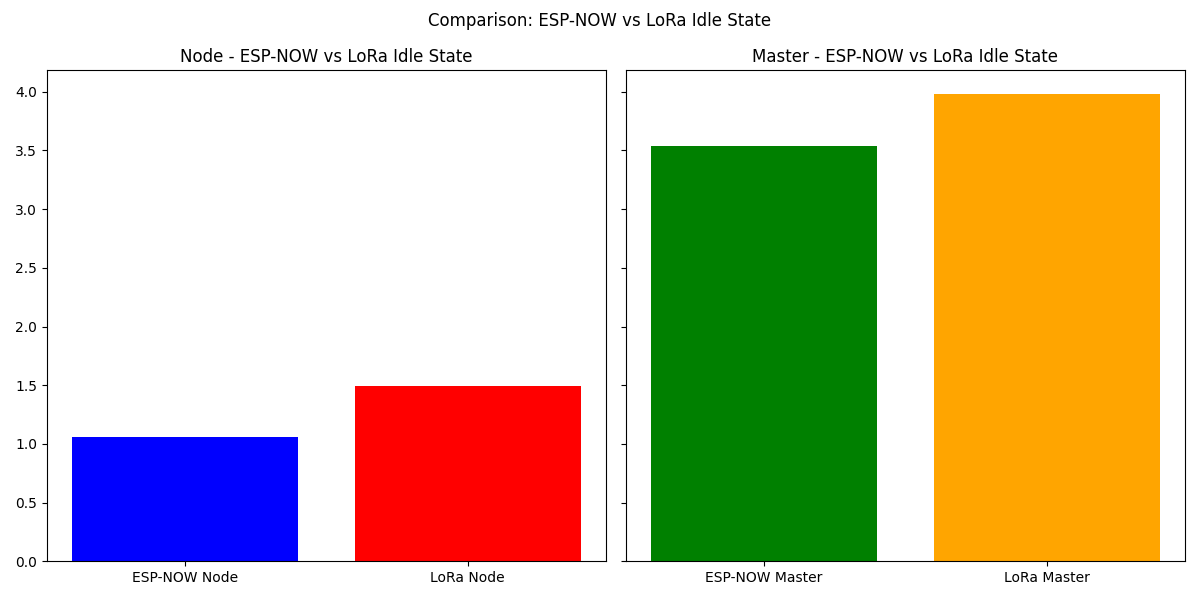
\includegraphics[width=0.45\textwidth]{./Figures/Average_Power_Consumption/ESP-NOW_vs_LORA_Idle.png}
  \end{center}
  \caption{Idle State of ESP-NOW VS LORA}\label{fig:esp_lora_idle}
\end{figure}

Figure \ref{fig:esp_lora_idle} shows that ESP-NOW technology demonstrates lower power consumption in the idle state for both node and master configurations. This suggests that ESP-NOW is a more energy-efficient option when devices are not actively communicating. This aspect of power efficiency is especially advantageous in applications where devices are expected to operate on battery power for extended durations and spend a significant amount of time in the idle state. The reduced energy usage can lead to longer battery life and decreased operational costs, making ESP-NOW an attractive choice for energy-conscious wireless communication implementations.

\begin{figure}[H]
  \begin{center}
    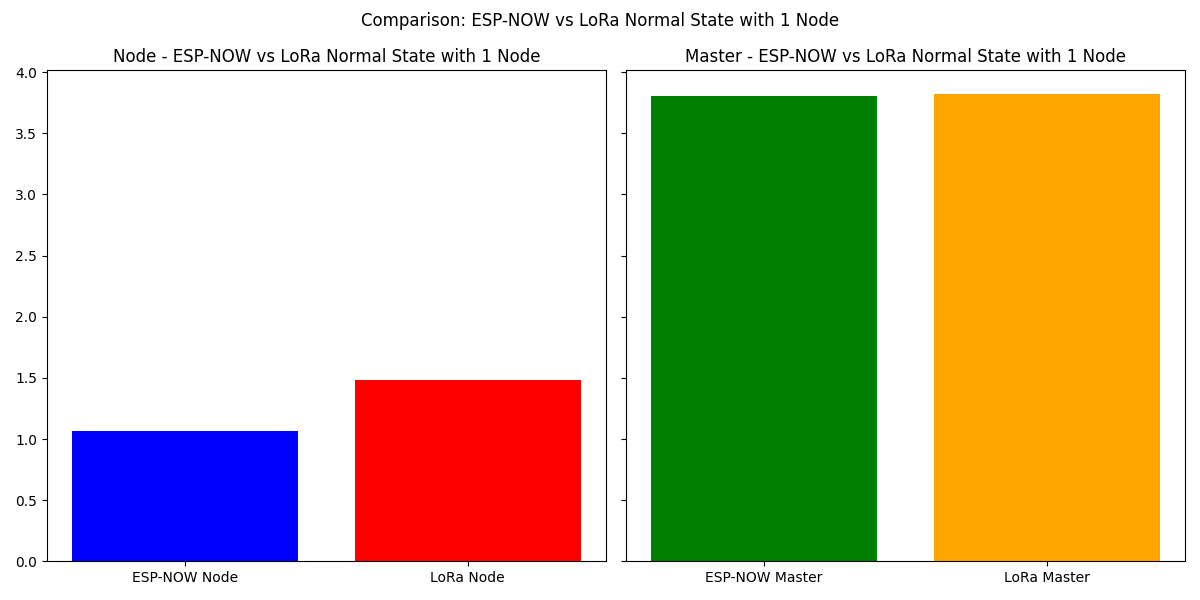
\includegraphics[width=0.45\textwidth]{./Figures/Average_Power_Consumption/ESP-NOW_vs_LORA_Normal_1_node.png}
  \end{center}
  \caption{Normal State with 1 node of ESP-NOW VS LORA}\label{fig:esp_lora_1}
\end{figure}

Figure \ref{fig:esp_lora_1} highlights the enhanced power efficiency of ESP-NOW in a single-node setup, where it outshines LoRa by registering a lower rate of power consumption, as illustrated by the blue bar for the ESP-NOW Node versus the red bar for the LoRa Node. This efficiency also extends to master nodes, where the ESP-NOW Master shows energy consumption that is nearly identical to that of the LoRa Master. The advantage of the ESP-NOW's lower power demand becomes particularly significant in configurations with a sole node, potentially extending the device's usable life and minimizing the need for frequent maintenance. The energy-conserving trait of ESP-NOW is also of paramount importance in applications where the power supply is constrained, such as with battery-operated sensors in isolated locations, making it a strategic choice for energy management.

\begin{figure}[H]
  \begin{center}
    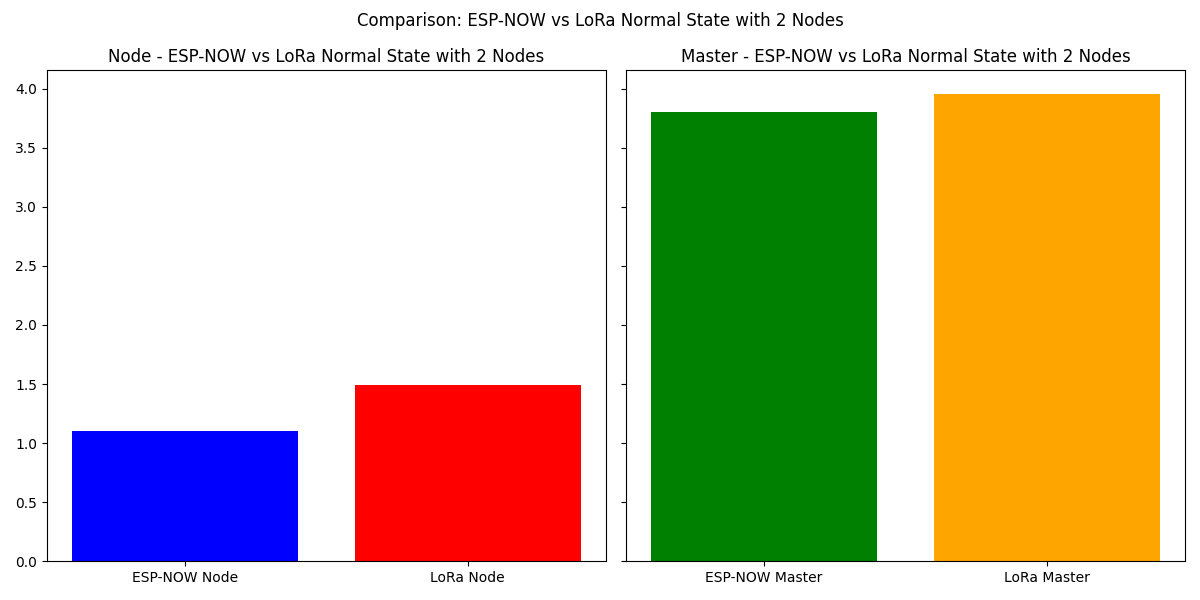
\includegraphics[width=0.45\textwidth]{./Figures/Average_Power_Consumption/ESP-NOW_vs_LORA_Normal_2_nodes.png}
  \end{center}
  \caption{Normal State with 2 nodes of ESP-NOW VS LORA}\label{fig:esp_lora_2}
\end{figure}

In the two-node scenario depicted in figure \ref{fig:esp_lora_2}, the ESP-NOW Node (blue bar) consumes less power than the LoRa Node (red bar), demonstrating ESP-NOW’s greater power efficiency. The Master nodes for both ESP-NOW (green bar) and LoRa (yellow bar) show similar power consumption, suggesting that for master nodes, the choice between ESP-NOW and LoRa may not significantly affect power usage. Overall, in a two-node system, ESP-NOW offers an advantage for individual nodes in terms of power efficiency.

\begin{figure}[H]
  \begin{center}
    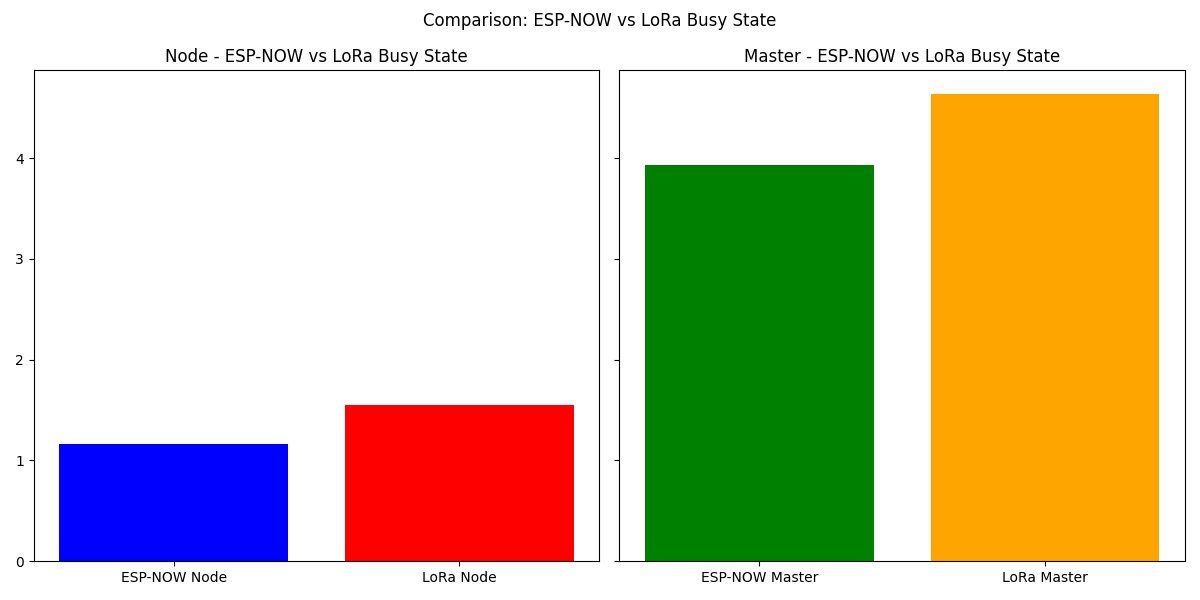
\includegraphics[width=0.45\textwidth]{./Figures/Average_Power_Consumption/ESP-NOW_vs_LORA_Busy.png}
  \end{center}
  \caption{Busy State of ESP-NOW VS LORA}\label{fig:esp_lora_busy}
\end{figure}

Figure \ref{fig:esp_lora_busy} depicts a busy state scenario, ESP-NOW technology (blue bar) still maintains lower power consumption compared to LoRa (red bar) for individual nodes. This indicates that even when the network is busy with higher levels of communication and data transmission, ESP-NOW nodes operate more efficiently than LoRa nodes.

For master nodes, the ESP-NOW Master (green bar) consumes significantly less power than the LoRa Master (yellow bar). In a busy network state, this difference suggests that ESP-NOW is notably more power-efficient for master nodes as well. The graph reflects that in high-activity situations, where nodes and masters are frequently communicating, ESP-NOW's power efficiency is a substantial advantage.

% Summary of analysis
\subsection{Summary of Analysis}\label{analysis_summary}

In terms of performance within a wireless sensor network with four nodes, the ESP-NOW protocol surpasses LoRa with a higher throughput of 6.0261 packets per second against 1.789 packets per second for LoRa. It also benefits from considerably lower latency at approximately 0.165 seconds per packet compared to LoRa’s 1.676 seconds per packet and greater bandwidth at 180.78 bytes per second over LoRa’s 89.45 bytes per second. ESP-NOW’s capabilities make it preferable for high-speed, low-latency communication needs, while LoRa remains a viable choice for its long-range and obstacle penetration abilities.

Regarding power consumption, ESP-NOW showcases lower power usage than LoRa in both idle and active (busy) network states. For single-node configurations, ESP-NOW's power efficiency could lead to longer battery life and less frequent maintenance, beneficial for remote and battery-operated devices. In networks with two nodes, ESP-NOW nodes use less energy, though master node power consumption is similar between the protocols. Even under busy conditions, ESP-NOW sustains its power-saving benefits for individual and master nodes alike, indicating a significant advantage for energy-sensitive deployments.



